\documentclass[12pt]{article}
%\pagestyle{empty}
% NMD additions 
%\usepackage{graphicx, overpic}
\usepackage[colorlinks=true, linkcolor=blue, citecolor=blue]{hyperref}

% end NMD additions 
\usepackage[T1]{fontenc}

\setlength{\tabcolsep}{20pt}
\setlength{\topmargin}{0.5cm}
\setlength{\oddsidemargin}{-0.2cm}
\setlength{\evensidemargin}{-0.2cm}
\textheight = 22cm  
\textwidth = 16.2cm


\usepackage{enumerate, amsfonts, latexsym, color, url}
\usepackage[pdftex]{graphicx}
%\usepackage{epstopdf}

%\usepackage{pinlabel}


\begin{document}


\title{{\tt kleinian}; a GLUT program for visualizing Kleinian groups}

\author{Danny Calegari}
%\address{University of Chicago \\ Chicago, Ill 60637 USA}
%\email{dannyc@math.uchicago.edu}
\date{\today}


%\begin{abstract}
%\end{abstract}

\maketitle
\setcounter{tocdepth}{1}
\tableofcontents

\section{Summary}
This manual describes the GLUT program {\tt kleinian} and the 
format of the data files it takes. This program uses the GLUT
interface to display hyperbolic polyhedra (in the Poincar\'e ball model)
which are invariant under Kleinian groups. 

\begin{figure}[ht]
\centering
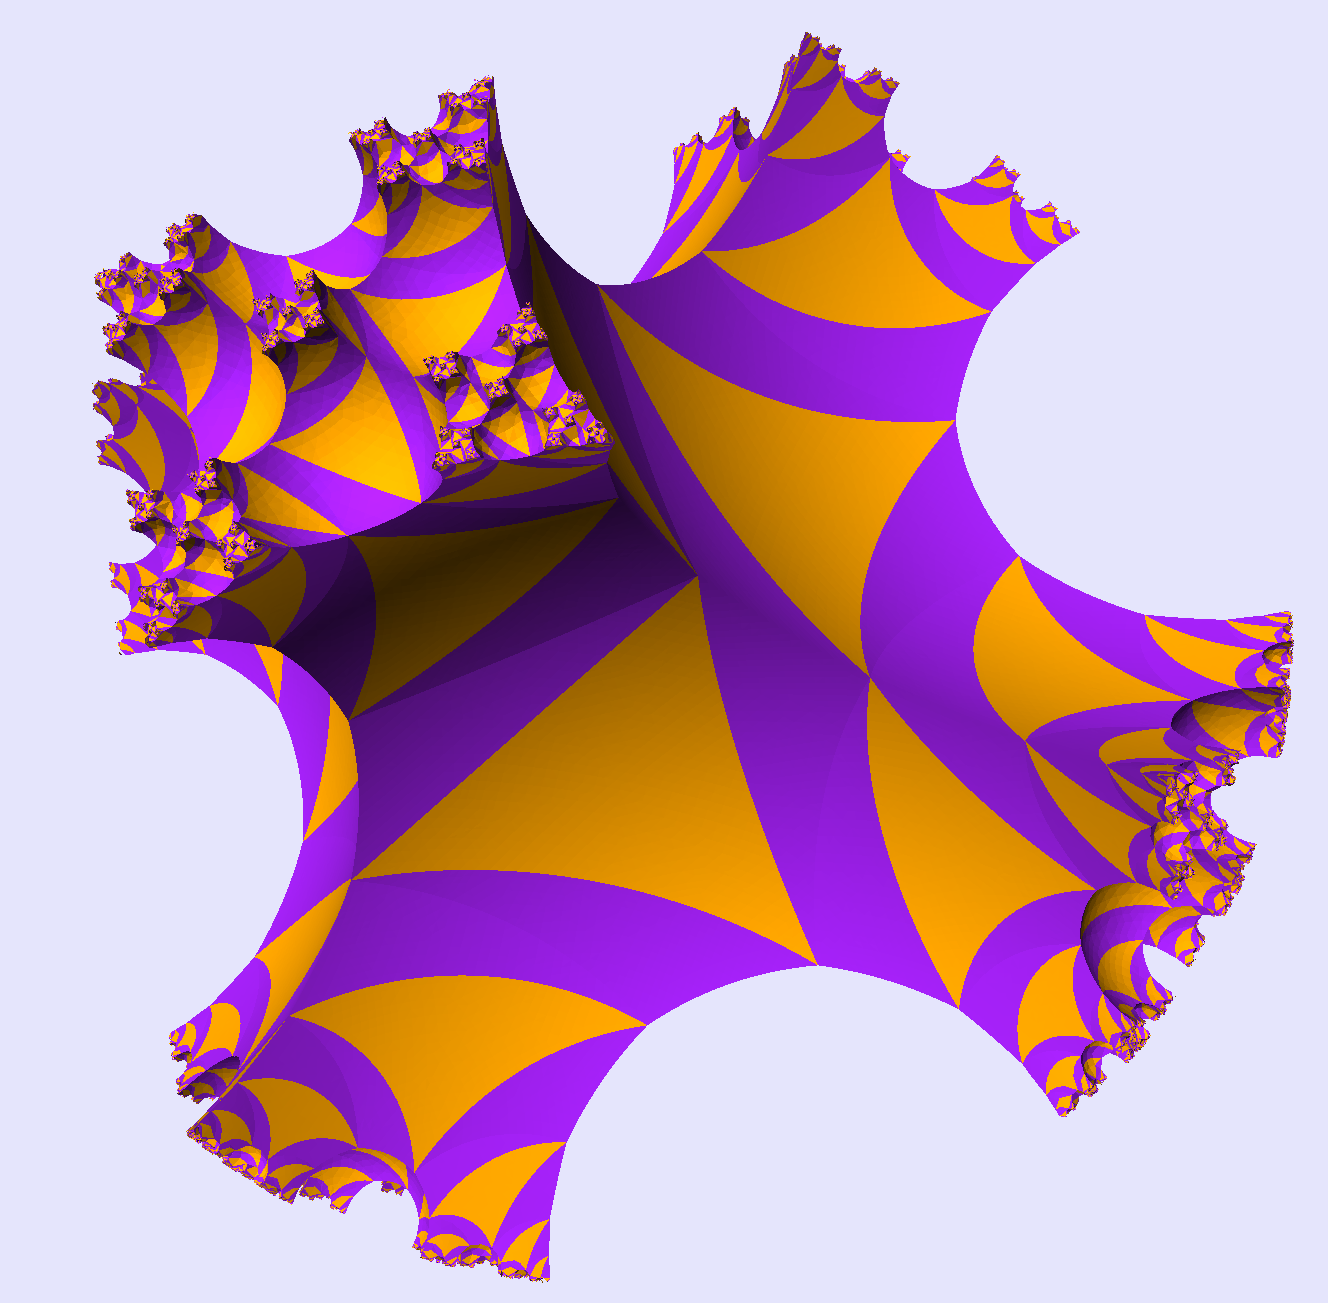
\includegraphics[width=0.75\textwidth]{example_pictures/schottky}
\caption{A domain invariant under a rank 3 Schottky group}\label{schottky}
\end{figure}

Figure~\ref{schottky} gives an example of a domain invariant under
a rank 3 Schottky group. The quotient is a genus 3 handlebody with
boundary decomposed into totally geodesic subsurfaces which meet at right
angles.

\section{Installing the program}\label{section:installation}

The program can be built on your local machine by following these instructions:

\begin{enumerate}
\item{Download the program files as a zip archive from github, from 
\url{http://github.com/dannycalegari/kleinian}.}
\item{Unzip the archive on your local computer; this should create a new folder containing
the source files, some examples, the source for this manual (as a \LaTeX file), and a
makefile.}
\item{The makefile assumes the user has the GNU c compiler ({\tt g++}) installed, and that the standard
X-windows include files and libraries are installed in the directories {\tt /usr/X11R6/include}
and {\tt /usr/X11R6/lib}, and the GLUT framework is available. 
Edit these values if necessary.}
\item{Make the program from the command line with the command {\tt make}.}
\end{enumerate}

The program has been built successfully on Macintosh computers running OS X.
It has also been successfully built on an Ubuntu Linux distribution; 
for this, the following modifications were necessary:

\begin{enumerate}
\item{changed {\tt -fast} to {\tt -Ofast} and added linker options
{\tt -lglut -lGLU -lGL} in makefile.}
\item{installed package {\tt freeglut3-dev}.}
\end{enumerate}

\section{Data formats}\label{section:data_format}

The program is run from the command line with one of the following
commands:
\begin{enumerate}
\item{{\tt ./kleinian -t {\sl filename.tri}} to read a precomputed triangle mesh from a file}
\item{{\tt ./kleinian -g {\sl filename.grp}} to read semigroup generators and triangle orbits from a file}
\item{{\tt ./kleinian -e} to run one of three hardcoded examples.}
\end{enumerate}

These options are explained below.

\subsection{Reading a precomputed triangle mesh}

A data file called {\sl filename.tri} in {\em triangle format} may be read with
the command {\tt ./kleinian -t {\sl filename.tri}}. This data file defines a
triangular mesh, which is displayed with GLUT. Note that these triangles are
Euclidean triangles; i.e.\/ the result of subdividing Poincar\'e triangles to
the mesh size to make the result appear curvilinear. Thus, if the mesh size is
small, or if there were many Poincar\'e triangles in the original mesh,
these files can be very large.

Triangle format is very simple: 
\begin{enumerate}
\item{The first line is the number $N$ of triangles.}
\item{The next $5N$ lines each have three numbers on them. In each group of 5 lines,
the first 3 lines are the $xyz$ coordinates of the triangle vertex, the next
line are the $xyz$ coordinates of the (unit) normal to the triangle, and the
last line is the rgb color of the triangle.}
\item{The last line is the rgb background color of the scene.}
\end{enumerate}

Here is a simple commented example:

\begin{center}
{\tt
\begin{tabular}{llll}
60 & & & 60 triangles \\
-0.904988 & 0.000000 & 0.000000 & triangle 0 vertex 0 \\
-0.719152 & 0.549384 & 0.000000 & triangle 0 vertex 1 \\
-0.719152 & 0.169769 & 0.522495 & triangle 0 vertex 2 \\
-0.922602 & 0.312081 & 0.22674  & normal to triangle 0 \\
0.913725 & 0.588235 & 0.47843 & rgb color of triangle 0 \\
\dots & & & \\
0.9 & 0.9 & 0.99 & rgb background color \\
\end{tabular}
}
\end{center}

Producing a data file in triangle format by hand is probably quite laborious;
note that all the program does with such a file is to display it using GLUT
primitives, and allow the user to rotate the result. Thus there is no
requirement that the mesh have anything to do with Kleinian groups or 
hyperbolic geometry, and this feature of the program could be used to visualize
triangular meshes of any origin.

When {\tt kleinian} is run in some other mode, the resulting triangular mesh
(which can take a long time to compute if it is very complicated or has very
small mesh size) can be saved as a file in triangle format, which can then
be loaded and displayed quickly. This is the main function of this mode and
format.

\subsection{Reading semigroup generators and triangle orbits}

A data file called {\sl filename.grp} in {\em group format} may be read with
the command {\tt ./kleinian -g {\sl filename.grp}}. This data file defines
a finite list of semigroup generators, and a finite number of (Poincar\'e)
triangle orbits. The program will read the generators, generate the Cayley
graph out to some depth, translate the triangle orbits about by 
list of generated matrix elements, project the Poincar\'e triangles to
curvilinear Euclidean triangles in the Poincar\'e ball model, and approximate
the result by a mesh of small Euclidean triangles which are then rendered
in GLUT mode.

Group format has the following structure:
\begin{enumerate}
\item{The first line is the number $N$ of semigroup generators.}
\item{The second line is either the character {\tt n} 
(for {\em numerical} format) or {\tt k} (for {\em algebraic} format).
\begin{itemize}
\item{In numerical format, the next $4N$ lines are the matrix entries of
the semigroup generators; these are matrices in $\textnormal{O}(3,1)$, and
each of the four lines corresponding to a generators is a row of the matrix.}
\item{In algebraic format, for each of the $N$ generators $G(i)$, there is an
integer $m(i)$ (the number of {\em elementary} generators whose product is the
$G(i)$), and then for $j=0$ to $m(i)-1$, a triple of the form
$a_j,b_j,l_j$ where $a_j$ and $b_j$ are distinct integers between $0$ and $3$, and
$l_j$ is a real number. Then 
$$G(i)=M(a_0,b_0,l_0)*M(a_1,b_1,l_1)*\cdots *M(a_{m(i)-1},b_{m(i)-1},l_{m(i)-1})$$
where $M(a,b,l)$ is a rotation through angle $l$ in the Euclidean $a$--$b$ plane
(when $a,b < 3$) and translation through hyperbolic distance $l$ along the
$a$ axis (when $a<3$ and $b=3$).}
\end{itemize}
}
\item{The next line is the number $M$ of triangle orbits.}
\item{For each of the next $3M$ lines, each triple of lines are the
coordinates of the vertices of the given triangle orbit. These are {\em Poincar\'e}
triangles, whose vertices are in Lorentz 4-space. Thus, each vertex 
coordinate is a 4-tuple $x,y,z,w$ satisfying $w^2-x^2-y^2-z^2=1$.}
\item{If the next line is the character {\tt c} then the next $M$ lines are
the rgb colors of the triangle orbits. Otherwise the color of all triangles
defaults to white.}
\item{If colors were specified, then if the next line is the character {\tt b}
the next line is the rgb background color. Otherwise the background color defaults
to light blue.}
\end{enumerate}

Here is an example in numerical format:

\begin{center}
{\footnotesize
{\tt
\begin{tabular}{lllll}
4 & & & & 4 generators \\
n & & & & numerical format \\
3.7621957 & 0.0000000 & 0.0000000 & 3.6268604 & generator 0 \\
0.0000000 & 1.0000000 & 0.0000000 & 0.0000000 & \\
0.0000000 & 0.0000000 & 1.0000000 & 0.0000000 & \\
3.6268604 & 0.0000000 & 0.0000000 & 3.7621957 & \\
\dots & & & & \\
1 & & & & 1 triangle orbit \\
1.81343 & 1.1752012 & 0.00000 & 2.3810978 & triangle vertex 0 \\
1.81343 & 0.00000 & 1.1752012 & 2.3810978 & triangle vertex 1 \\
1.1752012 & 1.81343 & 0.00000 & 2.3810978 & triangle vertex 2 \\
c & & & & triangle color \\
0.62745 & 0.12549 & 0.94117647 & & rgb value\\
b & & & & background color \\
0.9 & 0.9 & 0.99 & & rgb value \\
\end{tabular}
}
}
\end{center}

Here is an example in algebraic format:

\begin{center}
{\footnotesize
{\tt
\begin{tabular}{lllll}
4 & & & & 4 generators \\
k & & & & algebraic format \\
2 & & & & generator 0 has factors \\
0 & 3 & 0.54930614 & & translate x axis 0.549 \\
0 & 2 & -2.0943951 & & rotate xz-plane -2.094 \\
\dots & & & & \\
1 & & & & 1 triangle orbit \\
1.81343 & 1.1752012 & 0.00000 & 2.3810978 & triangle vertex 0 \\
1.81343 & 0.00000 & 1.1752012 & 2.3810978 & triangle vertex 1 \\
1.1752012 & 1.81343 & 0.00000 & 2.3810978 & triangle vertex 2 \\
c & & & & triangle color \\
0.62745 & 0.12549 & 0.94117647 & & rgb value\\
b & & & & background color \\
0.9 & 0.9 & 0.99 & & rgb value \\
\end{tabular}
}
}
\end{center}

\section{Program interface}\label{section:interface}

When the program reads a file in triangle format, it loads the mesh into
GLUT, and moves into GLUT mode.

When the program reads a file in group format, it begins a dialog with the
user to determine parameters. 
\begin{enumerate}
\item{First, the user is prompted to enter the depth to generate the Cayley
graph to. This should be a non-negative integer.
Unless the group is elementary (e.g.\/ a parabolic or finite group)
or the fundamental domain is very small (e.g.\/ a $2,3,7$ triangle group), this
should probably be 12 or less, unless very fine detail is needed.}
\item{After computing the Cayley graph out to the specified depth, the user
is asked whether they want fancy curvilinear triangles. The answer should be
a single character, either {\tt y} or {\tt n}.}
\item{An {\tt n} answer will make the triangles Euclidean, but their vertices
will be in the correct location for the Poincar\'e model. This is a reasonable
approximation when the triangles have small hyperbolic diameter, but will look
terrible if some triangles are (almost) ideal.}
\item{A {\tt y} answer will prompt the user to supply a mesh size to subdivide
the triangles to. This should be a floating point number, generally between
$0.02$ and $0.2$. If the mesh is too small, and some triangles are too big, the
program might run into numerical difficulty and crash.}
\item{The program then computes the subdivided triangle mesh, and enters GLUT mode.}
\end{enumerate}

When the program is run in example mode, the user can select one of three
pre-computed examples to run, and for each they might first be prompted for
some parameters of the example, before starting the dialog above.

\subsection{GLUT mode}

In GLUT mode, the following keypress options are available:
\begin{itemize}
\item{[arrow keys] rotate the display}
\item{[t] saves the triangulation to {\sl output\_file.tri}}
\item{[g] saves the generators (e.g. in example mode) to {\sl output\_file.grp}}
\item{[e] saves the figure as an .eps file {\sl output.eps}}
\item{[command-q] exits the program.}
\end{itemize}

\section{Acknowledgments}
Danny Calegari is partially supported by NSF grant DMS 1005246. The program 
{\tt kleinian} is released under the terms of the GNU GPL License version 3.0.

\medskip

\noindent Version 0.01 of {\tt kleinian} was released February 28, 2014 
and is copyright Danny Calegari.

\begin{figure}[ht]
\centering
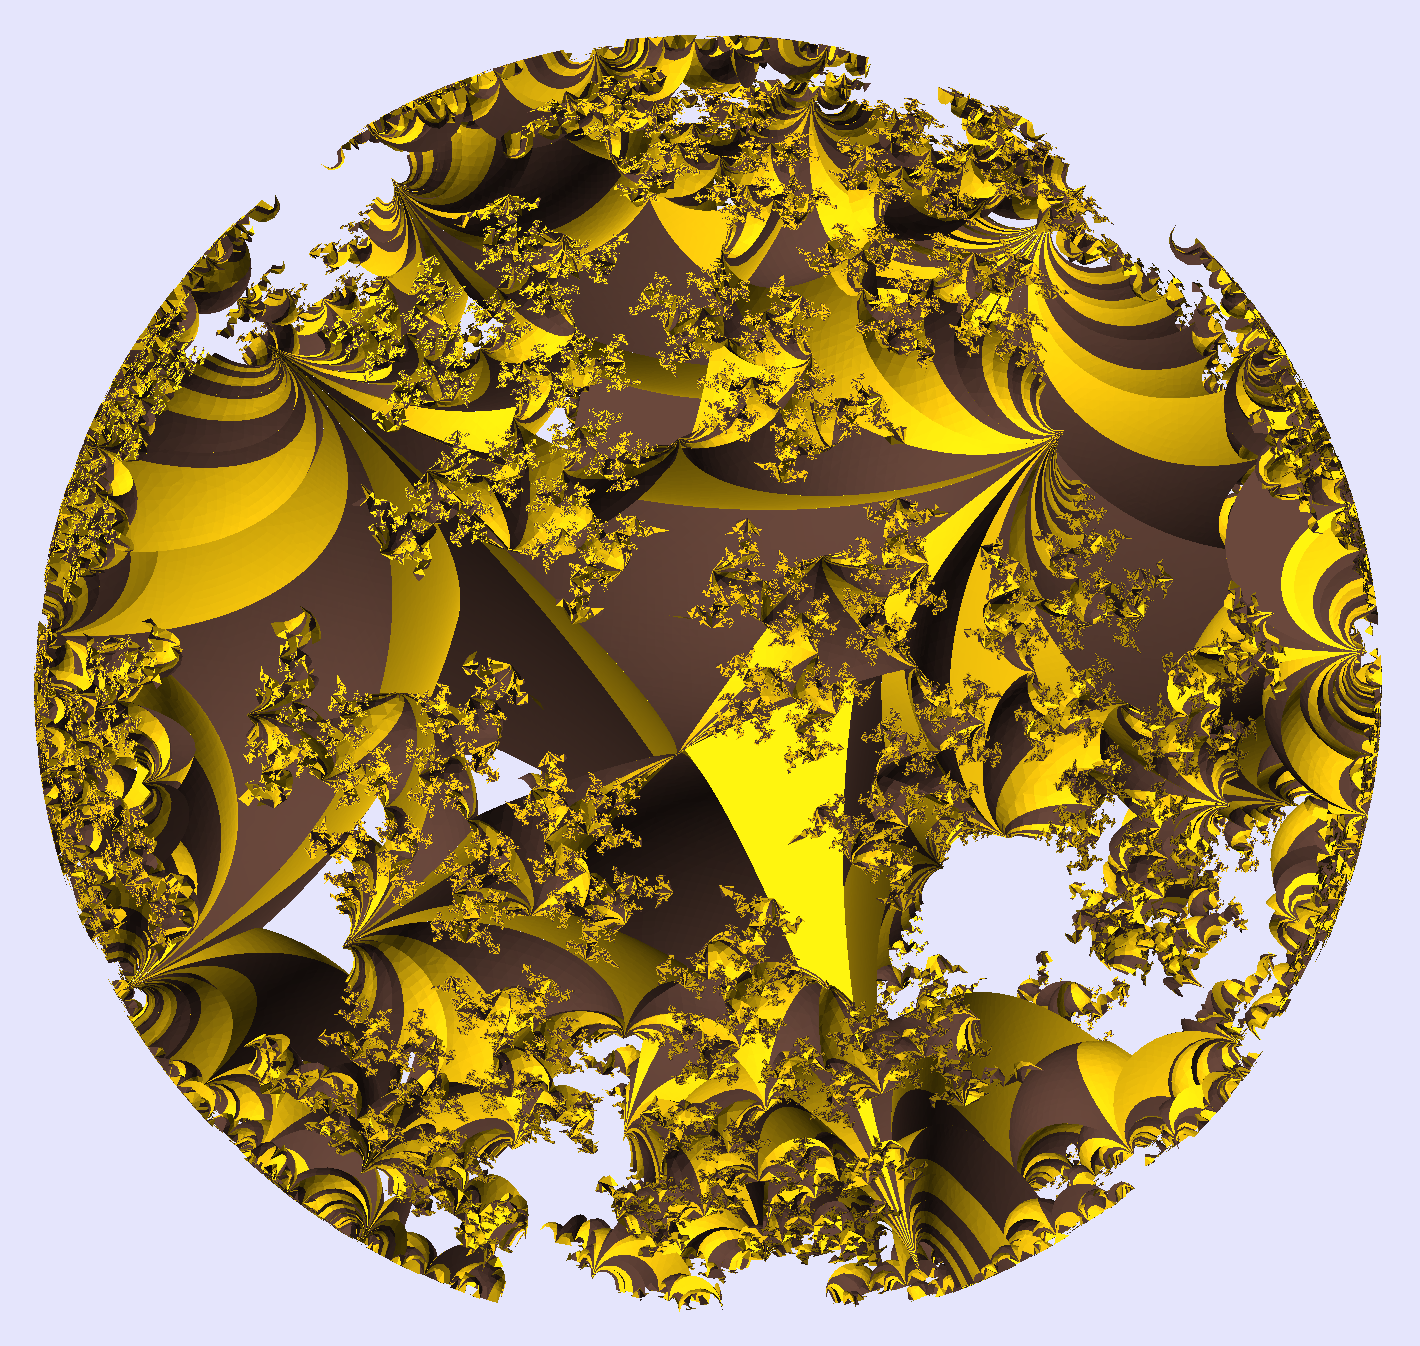
\includegraphics[width=0.75\textwidth]{example_pictures/fiber}
\caption{Figure 8
knot fiber}\label{fiber}
\end{figure}

\end{document}